% Options for packages loaded elsewhere
\PassOptionsToPackage{unicode}{hyperref}
\PassOptionsToPackage{hyphens}{url}
%
\documentclass[
]{article}
\usepackage{lmodern}
\usepackage{amssymb,amsmath}
\usepackage{ifxetex,ifluatex}
\ifnum 0\ifxetex 1\fi\ifluatex 1\fi=0 % if pdftex
  \usepackage[T1]{fontenc}
  \usepackage[utf8]{inputenc}
  \usepackage{textcomp} % provide euro and other symbols
\else % if luatex or xetex
  \usepackage{unicode-math}
  \defaultfontfeatures{Scale=MatchLowercase}
  \defaultfontfeatures[\rmfamily]{Ligatures=TeX,Scale=1}
\fi
% Use upquote if available, for straight quotes in verbatim environments
\IfFileExists{upquote.sty}{\usepackage{upquote}}{}
\IfFileExists{microtype.sty}{% use microtype if available
  \usepackage[]{microtype}
  \UseMicrotypeSet[protrusion]{basicmath} % disable protrusion for tt fonts
}{}
\makeatletter
\@ifundefined{KOMAClassName}{% if non-KOMA class
  \IfFileExists{parskip.sty}{%
    \usepackage{parskip}
  }{% else
    \setlength{\parindent}{0pt}
    \setlength{\parskip}{6pt plus 2pt minus 1pt}}
}{% if KOMA class
  \KOMAoptions{parskip=half}}
\makeatother
\usepackage{xcolor}
\IfFileExists{xurl.sty}{\usepackage{xurl}}{} % add URL line breaks if available
\IfFileExists{bookmark.sty}{\usepackage{bookmark}}{\usepackage{hyperref}}
\hypersetup{
  pdftitle={Barack Obama Retweets Network},
  pdfauthor={Mateusz Zaremba},
  hidelinks,
  pdfcreator={LaTeX via pandoc}}
\urlstyle{same} % disable monospaced font for URLs
\usepackage[margin=1.5in]{geometry}
\usepackage{color}
\usepackage{fancyvrb}
\newcommand{\VerbBar}{|}
\newcommand{\VERB}{\Verb[commandchars=\\\{\}]}
\DefineVerbatimEnvironment{Highlighting}{Verbatim}{commandchars=\\\{\}}
% Add ',fontsize=\small' for more characters per line
\usepackage{framed}
\definecolor{shadecolor}{RGB}{248,248,248}
\newenvironment{Shaded}{\begin{snugshade}}{\end{snugshade}}
\newcommand{\AlertTok}[1]{\textcolor[rgb]{0.94,0.16,0.16}{#1}}
\newcommand{\AnnotationTok}[1]{\textcolor[rgb]{0.56,0.35,0.01}{\textbf{\textit{#1}}}}
\newcommand{\AttributeTok}[1]{\textcolor[rgb]{0.77,0.63,0.00}{#1}}
\newcommand{\BaseNTok}[1]{\textcolor[rgb]{0.00,0.00,0.81}{#1}}
\newcommand{\BuiltInTok}[1]{#1}
\newcommand{\CharTok}[1]{\textcolor[rgb]{0.31,0.60,0.02}{#1}}
\newcommand{\CommentTok}[1]{\textcolor[rgb]{0.56,0.35,0.01}{\textit{#1}}}
\newcommand{\CommentVarTok}[1]{\textcolor[rgb]{0.56,0.35,0.01}{\textbf{\textit{#1}}}}
\newcommand{\ConstantTok}[1]{\textcolor[rgb]{0.00,0.00,0.00}{#1}}
\newcommand{\ControlFlowTok}[1]{\textcolor[rgb]{0.13,0.29,0.53}{\textbf{#1}}}
\newcommand{\DataTypeTok}[1]{\textcolor[rgb]{0.13,0.29,0.53}{#1}}
\newcommand{\DecValTok}[1]{\textcolor[rgb]{0.00,0.00,0.81}{#1}}
\newcommand{\DocumentationTok}[1]{\textcolor[rgb]{0.56,0.35,0.01}{\textbf{\textit{#1}}}}
\newcommand{\ErrorTok}[1]{\textcolor[rgb]{0.64,0.00,0.00}{\textbf{#1}}}
\newcommand{\ExtensionTok}[1]{#1}
\newcommand{\FloatTok}[1]{\textcolor[rgb]{0.00,0.00,0.81}{#1}}
\newcommand{\FunctionTok}[1]{\textcolor[rgb]{0.00,0.00,0.00}{#1}}
\newcommand{\ImportTok}[1]{#1}
\newcommand{\InformationTok}[1]{\textcolor[rgb]{0.56,0.35,0.01}{\textbf{\textit{#1}}}}
\newcommand{\KeywordTok}[1]{\textcolor[rgb]{0.13,0.29,0.53}{\textbf{#1}}}
\newcommand{\NormalTok}[1]{#1}
\newcommand{\OperatorTok}[1]{\textcolor[rgb]{0.81,0.36,0.00}{\textbf{#1}}}
\newcommand{\OtherTok}[1]{\textcolor[rgb]{0.56,0.35,0.01}{#1}}
\newcommand{\PreprocessorTok}[1]{\textcolor[rgb]{0.56,0.35,0.01}{\textit{#1}}}
\newcommand{\RegionMarkerTok}[1]{#1}
\newcommand{\SpecialCharTok}[1]{\textcolor[rgb]{0.00,0.00,0.00}{#1}}
\newcommand{\SpecialStringTok}[1]{\textcolor[rgb]{0.31,0.60,0.02}{#1}}
\newcommand{\StringTok}[1]{\textcolor[rgb]{0.31,0.60,0.02}{#1}}
\newcommand{\VariableTok}[1]{\textcolor[rgb]{0.00,0.00,0.00}{#1}}
\newcommand{\VerbatimStringTok}[1]{\textcolor[rgb]{0.31,0.60,0.02}{#1}}
\newcommand{\WarningTok}[1]{\textcolor[rgb]{0.56,0.35,0.01}{\textbf{\textit{#1}}}}
\usepackage{longtable,booktabs}
% Correct order of tables after \paragraph or \subparagraph
\usepackage{etoolbox}
\makeatletter
\patchcmd\longtable{\par}{\if@noskipsec\mbox{}\fi\par}{}{}
\makeatother
% Allow footnotes in longtable head/foot
\IfFileExists{footnotehyper.sty}{\usepackage{footnotehyper}}{\usepackage{footnote}}
\makesavenoteenv{longtable}
\usepackage{graphicx}
\makeatletter
\def\maxwidth{\ifdim\Gin@nat@width>\linewidth\linewidth\else\Gin@nat@width\fi}
\def\maxheight{\ifdim\Gin@nat@height>\textheight\textheight\else\Gin@nat@height\fi}
\makeatother
% Scale images if necessary, so that they will not overflow the page
% margins by default, and it is still possible to overwrite the defaults
% using explicit options in \includegraphics[width, height, ...]{}
\setkeys{Gin}{width=\maxwidth,height=\maxheight,keepaspectratio}
% Set default figure placement to htbp
\makeatletter
\def\fps@figure{htbp}
\makeatother
\setlength{\emergencystretch}{3em} % prevent overfull lines
\providecommand{\tightlist}{%
  \setlength{\itemsep}{0pt}\setlength{\parskip}{0pt}}
\setcounter{secnumdepth}{5}
\usepackage[]{natbib}
\bibliographystyle{plainnat}

\title{Barack Obama Retweets Network}
\author{Mateusz Zaremba}
\date{December 16, 2019}

\begin{document}
\maketitle

\hypertarget{introduction}{%
\section{Introduction}\label{introduction}}

In this report I will present a dataset obtained from the from
\url{http://networkrepository.com/rt-barackobama.php} website; it is a
retweet network of the US president Barack Obama. The network was
downloaded in a form of an edge list.

I wanted to see if by performing a set of tests on the network, it would
be possible to identify Barack Obama's vertex. I believe I succeded to
identify the aformnetioned vertex with a considerable degree of
confidence. I will present my reasoning and methods which led to me to
such conclusion.

--\textgreater{}

\hypertarget{methods}{%
\section{Methods}\label{methods}}

The network was analysed using R and Python programming languages, and
Gephi software package. The data statistics were calculated using
Python; the data preparation and manipulation was done using R; the data
visualisation was done using R and Gephi.

\hypertarget{data-preparation}{%
\subsection{Data Preparation}\label{data-preparation}}

The data was prepared using R programming language and RStudio software;
the data was downloaded, unziped and saved into a R table (within the
code). \emph{Timestamp} column was dropped (it would be useful if the
dataset was an updatable one; then it could be used to update the set
only from a certain timestamp but in this case the set was a complete
one).

By default, R names the columns like this:

\[  x =  \big\{V1, V2, ... , VN \mid N \in \mathbb{N} \big\}  \]

To make the data manipulation easier the columns were renamed such that:
\textbar{} Previous column name \textbar{} Current column name
\textbar{} \textbar{} - \textbar{} - \textbar{} \textbar{} V1 \textbar{}
from \textbar{} \textbar{} V2 \textbar{} to \textbar{}

Later, the data was saved in a \texttt{.csv} format so it could be easly
loaded into memory using Python programming language.

\hypertarget{metadata}{%
\subsection{Metadata}\label{metadata}}

The following metadata can be found on the
\url{http://networkrepository.com/rt-barackobama.php} website:

\hypertarget{network-size-metrics}{%
\subsection{Network size metrics}\label{network-size-metrics}}

The following metrics were used to analyse the data:

On the `Network Repository' website we can find already calculated
network data statistics, like number of nodes, number of edges, average
degree etc.; (Rossi and Ahmed, 2015). I created a network graph in
python programming language using networkx library and compared the
obtained statistics with the ones from the website; turns out they were
exactly the same, which gave me confidence that I prepared the data
correctly.

\begin{longtable}[]{@{}lll@{}}
\caption{The results are the same - we can be pretty confident we have
created our network graph in python correctly.}\tabularnewline
\toprule
& Calculated Statistics & Website Statistics\tabularnewline
\midrule
\endfirsthead
\toprule
& Calculated Statistics & Website Statistics\tabularnewline
\midrule
\endhead
Number of nodes & 9631 & 9.6K\tabularnewline
Number of edges & 9775 & 9.8K\tabularnewline
Average degree & 2.0299 & 2\tabularnewline
\bottomrule
\end{longtable}

\hypertarget{network-structure-metrics}{%
\subsection{Network Structure Metrics}\label{network-structure-metrics}}

Our graph in undirected so it does not contain in- or out-degrees.
Instead, we found the highest degree node - it had an id of 2506 and
degree of 7655; this was likely Barack Obama's twitter account since it
is the most connected.

\hypertarget{network-density}{%
\subsection{Network Density}\label{network-density}}

The network's density is equal to 0.000210789557302036, which is close
to zero, meaning - our graph is close to being `fully disconnected'.

\hypertarget{shortest-path-between-two-nodes}{%
\subsection{Shortest Path Between Two
Nodes}\label{shortest-path-between-two-nodes}}

We will find the shortest path between top two nodes with the highest
degree and between the nodes with the highest and the lowest degree.

\hypertarget{top-two}{%
\subsubsection{Top Two}\label{top-two}}

The top two nodes with the highest degree had ids: 2506 (Barack Obama)
and 9302. Shortest path between these two nodes is: {[}`2506', `8474',
`9302'{]}; the length of this path is 2, which means they are not
connected directly.

\hypertarget{highest-and-lowest-degree}{%
\subsubsection{Highest and Lowest
Degree}\label{highest-and-lowest-degree}}

As already mentioned, the id of the node with the highest degree is:
2506 and the id of the node with the lowest degree is: 2709; the
shortest path between these two nodes is: {[}`2506', `2709'{]} and its
length is 1, meaning the nodes are connected directly.

\hypertarget{identifying-network-communities}{%
\subsection{Identifying Network
Communities}\label{identifying-network-communities}}

We managed to identify 138 community groups:

\texttt{Counter(\{1:\ 7414,\ 6:\ 611,\ 7:\ 158,\ 12:\ 114,\ 4:\ 106,\ 2:\ 102,\ 50:\ 84,\ 5:\ 69,\ 88:\ 66,\ 61:\ 61,\ 127:\ 53,\ 35:\ 49,\ 19:\ 39,\ 25:\ 38,\ 17:\ 27,\ 111:\ 27,\ 77:\ 26,\ 23:\ 25,\ 112:\ 25,\ 0:\ 22,\ 49:\ 22,\ 26:\ 20,\ 54:\ 15,\ 37:\ 14,\ 102:\ 14,\ 22:\ 13,\ 41:\ 12,\ 48:\ 12,\ 55:\ 12,\ 9:\ 11,\ 15:\ 10,\ 32:\ 10,\ 75:\ 10,\ 97:\ 10,\ 34:\ 9,\ 38:\ 9,\ 82:\ 9,\ 85:\ 9,\ 13:\ 8,\ 3:\ 7,\ 29:\ 7,\ 84:\ 7,\ 105:\ 7,\ 108:\ 7,\ 68:\ 6,\ 78:\ 6,\ 83:\ 6,\ 117:\ 6,\ 86:\ 5,\ 110:\ 5,\ 8:\ 4,\ 27:\ 4,\ 31:\ 4,\ 62:\ 4,\ 67:\ 4,\ 79:\ 4,\ 93:\ 4,\ 100:\ 4,\ 129:\ 4,\ 10:\ 3,\ 20:\ 3,\ 36:\ 3,\ 40:\ 3,\ 47:\ 3,\ 66:\ 3,\ 70:\ 3,\ 80:\ 3,\ 81:\ 3,\ 87:\ 3,\ 90:\ 3,\ 95:\ 3,\ 104:\ 3,\ 107:\ 3,\ 114:\ 3,\ 125:\ 3,\ 133:\ 3,\ 134:\ 3,\ 139:\ 3,\ 11:\ 2,\ 14:\ 2,\ 16:\ 2,\ 18:\ 2,\ 21:\ 2,\ 24:\ 2,\ 28:\ 2,\ 30:\ 2,\ 33:\ 2,\ 39:\ 2,\ 42:\ 2,\ 43:\ 2,\ 44:\ 2,\ 45:\ 2,\ 46:\ 2,\ 51:\ 2,\ 52:\ 2,\ 53:\ 2,\ 56:\ 2,\ 57:\ 2,\ 58:\ 2,\ 59:\ 2,\ 60:\ 2,\ 63:\ 2,\ 64:\ 2,\ 65:\ 2,\ 69:\ 2,\ 71:\ 2,\ 72:\ 2,\ 73:\ 2,\ 74:\ 2,\ 76:\ 2,\ 89:\ 2,\ 91:\ 2,\ 92:\ 2,\ 94:\ 2,\ 96:\ 2,\ 98:\ 2,\ 99:\ 2,\ 101:\ 2,\ 103:\ 2,\ 106:\ 2,\ 109:\ 2,\ 113:\ 2,\ 115:\ 2,\ 116:\ 2,\ 118:\ 2,\ 119:\ 2,\ 120:\ 2,\ 121:\ 2,\ 122:\ 2,\ 123:\ 2,\ 124:\ 2,\ 126:\ 2,\ 128:\ 2,\ 130:\ 2,\ 131:\ 2,\ 132:\ 2,\ 135:\ 2,\ 136:\ 2,\ 137:\ 2,\ 138:\ 2\})}

It was calculated that the sizes of the communities range from 2 to
7414. We can, again, assume that the biggest community is likely to be
centred around Barack Obama.

\hypertarget{network-structure-connectivity}{%
\subsection{Network Structure
Connectivity}\label{network-structure-connectivity}}

Investigation reveals that the Barack Obama network is fully connected,
and it has no sub-components; this is not surprising because the edges
are retweets, nodes are twitter users and the network consists only of
users who retweeted Barack Obama's posts.

\hypertarget{network-hubsbrokers}{%
\subsection{Network Hubs/Brokers}\label{network-hubsbrokers}}

Betweenness and closeness centrality was successfully calculated
(Although, it took almost 40 minutes to compute) and sorted from the
highest to the lowest score for top 20 results; but a
\texttt{(PowerIterationFailedConvergence(...),\ \textquotesingle{}power\ iteration\ failed\ to\ converge\ within\ 100\ iterations\textquotesingle{})}
error kept occurring when calculating the nodes eigenvector centrality;
replacing \texttt{nx.eigenvector\_centrality} with
\texttt{nx.eigenvector\_centrality\_numpy} solved the issue (Stack
Overflow, 2019) and after the fix, the computation was almost
instantaneous.

Barack Obama's node (id = 2506) had the highest score in closeness,
betweenness and eigenvector centrality, which means:

\begin{itemize}
\tightlist
\item
  The highest closeness centrality score -- it is the farthest away from
  all other nodes in the network or -- it takes the most time to spread
  information sequentially from it to other nodes (Sciencedirect.com,
  2019).
\item
  The highest betweenness centrality score -- it has the highest number
  of distinct paths that strictly contain it in-between (Sci.unich.it,
  2019).
\item
  The highest eigenvector centrality score -- it is the most influential
  node in the network.
\end{itemize}

\hypertarget{results}{%
\section{Results}\label{results}}

It was also assumed that the biggest community of 7414 would be Barack
Obama's first-degree neighbours. This cannot be really well seen on the
graph without any colouring or sizing:

\begin{center}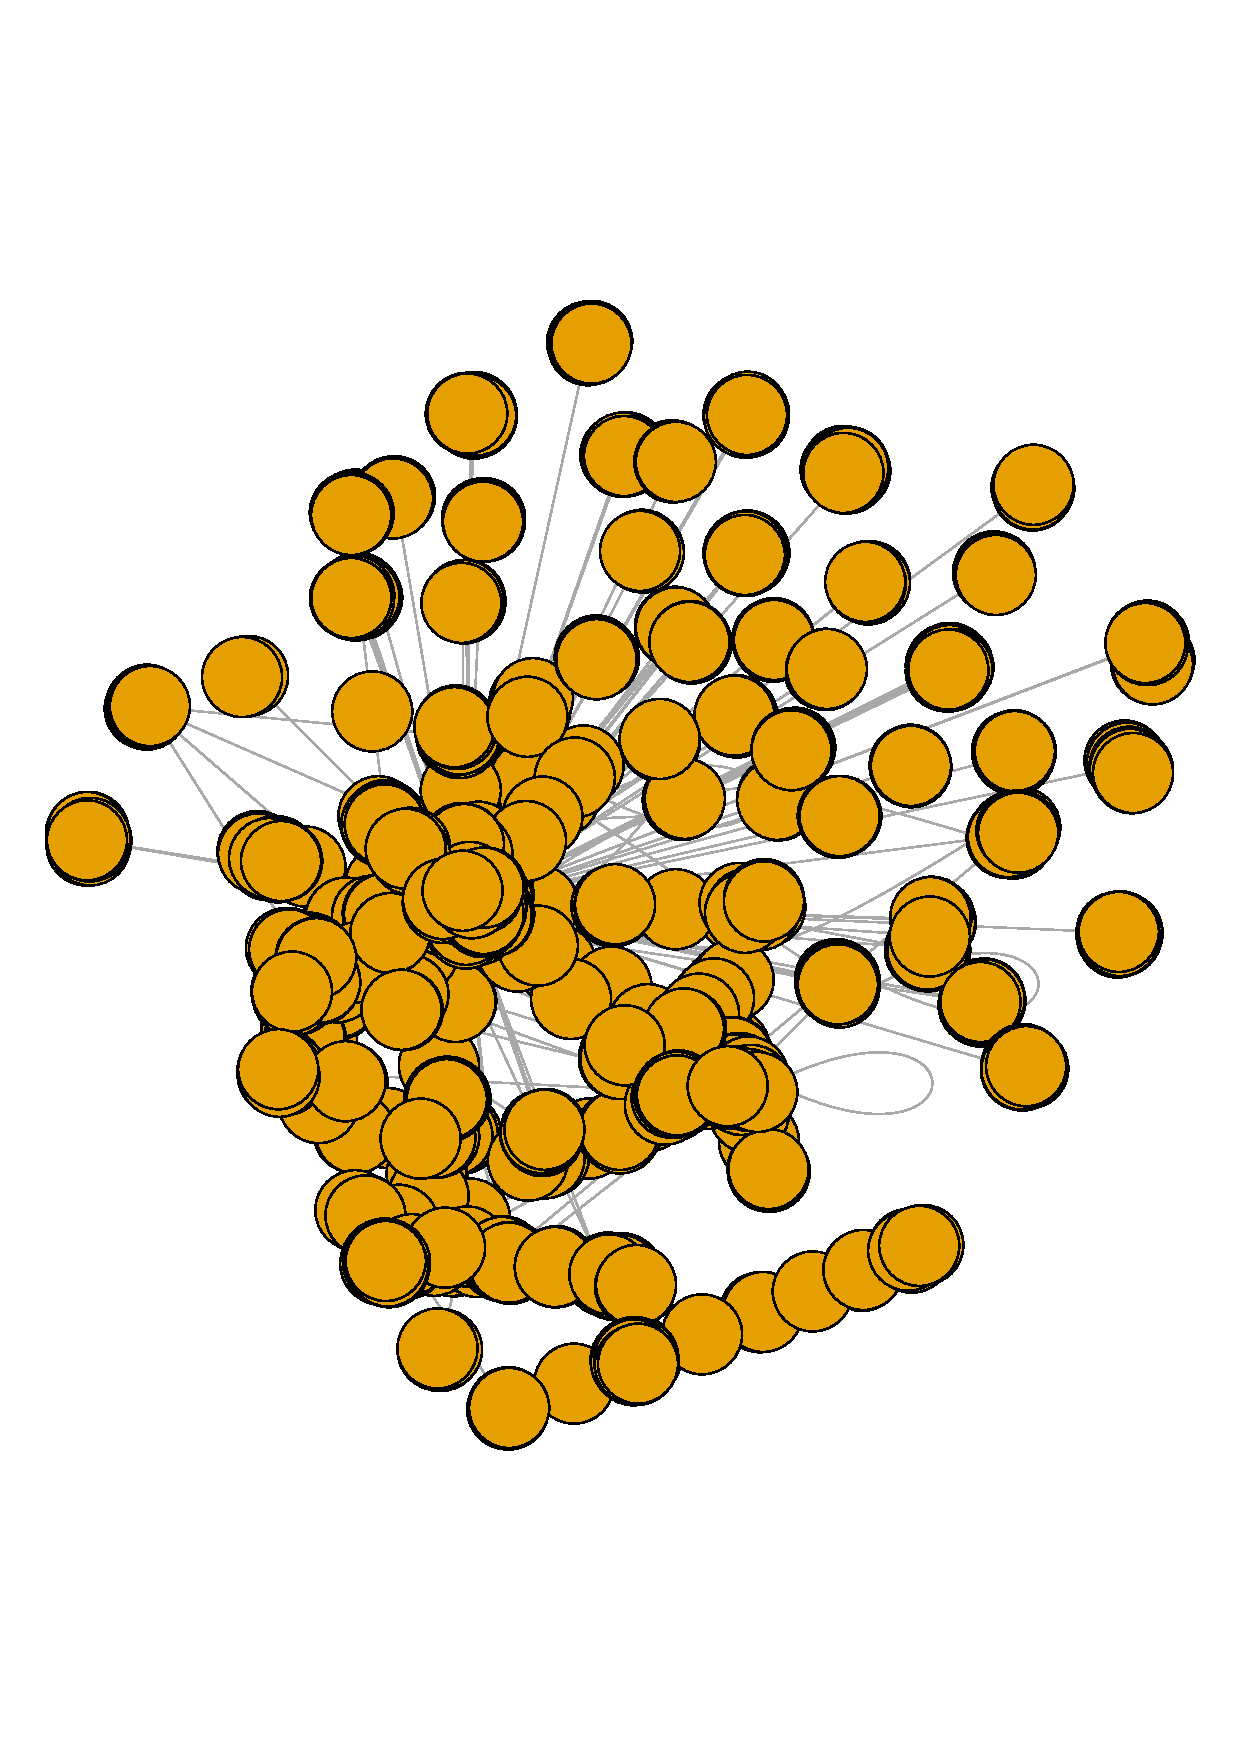
\includegraphics[width=0.55\linewidth]{/Users/mateuszzaremba/dev/R/Networks/Network/vanilla} \end{center}

But we can immediately see Barack Obama's node (The big red one,
obstructed by a bunch of smaller, blue nodes) when we distinguish the
node's degree using sizing and colouring:

\begin{center}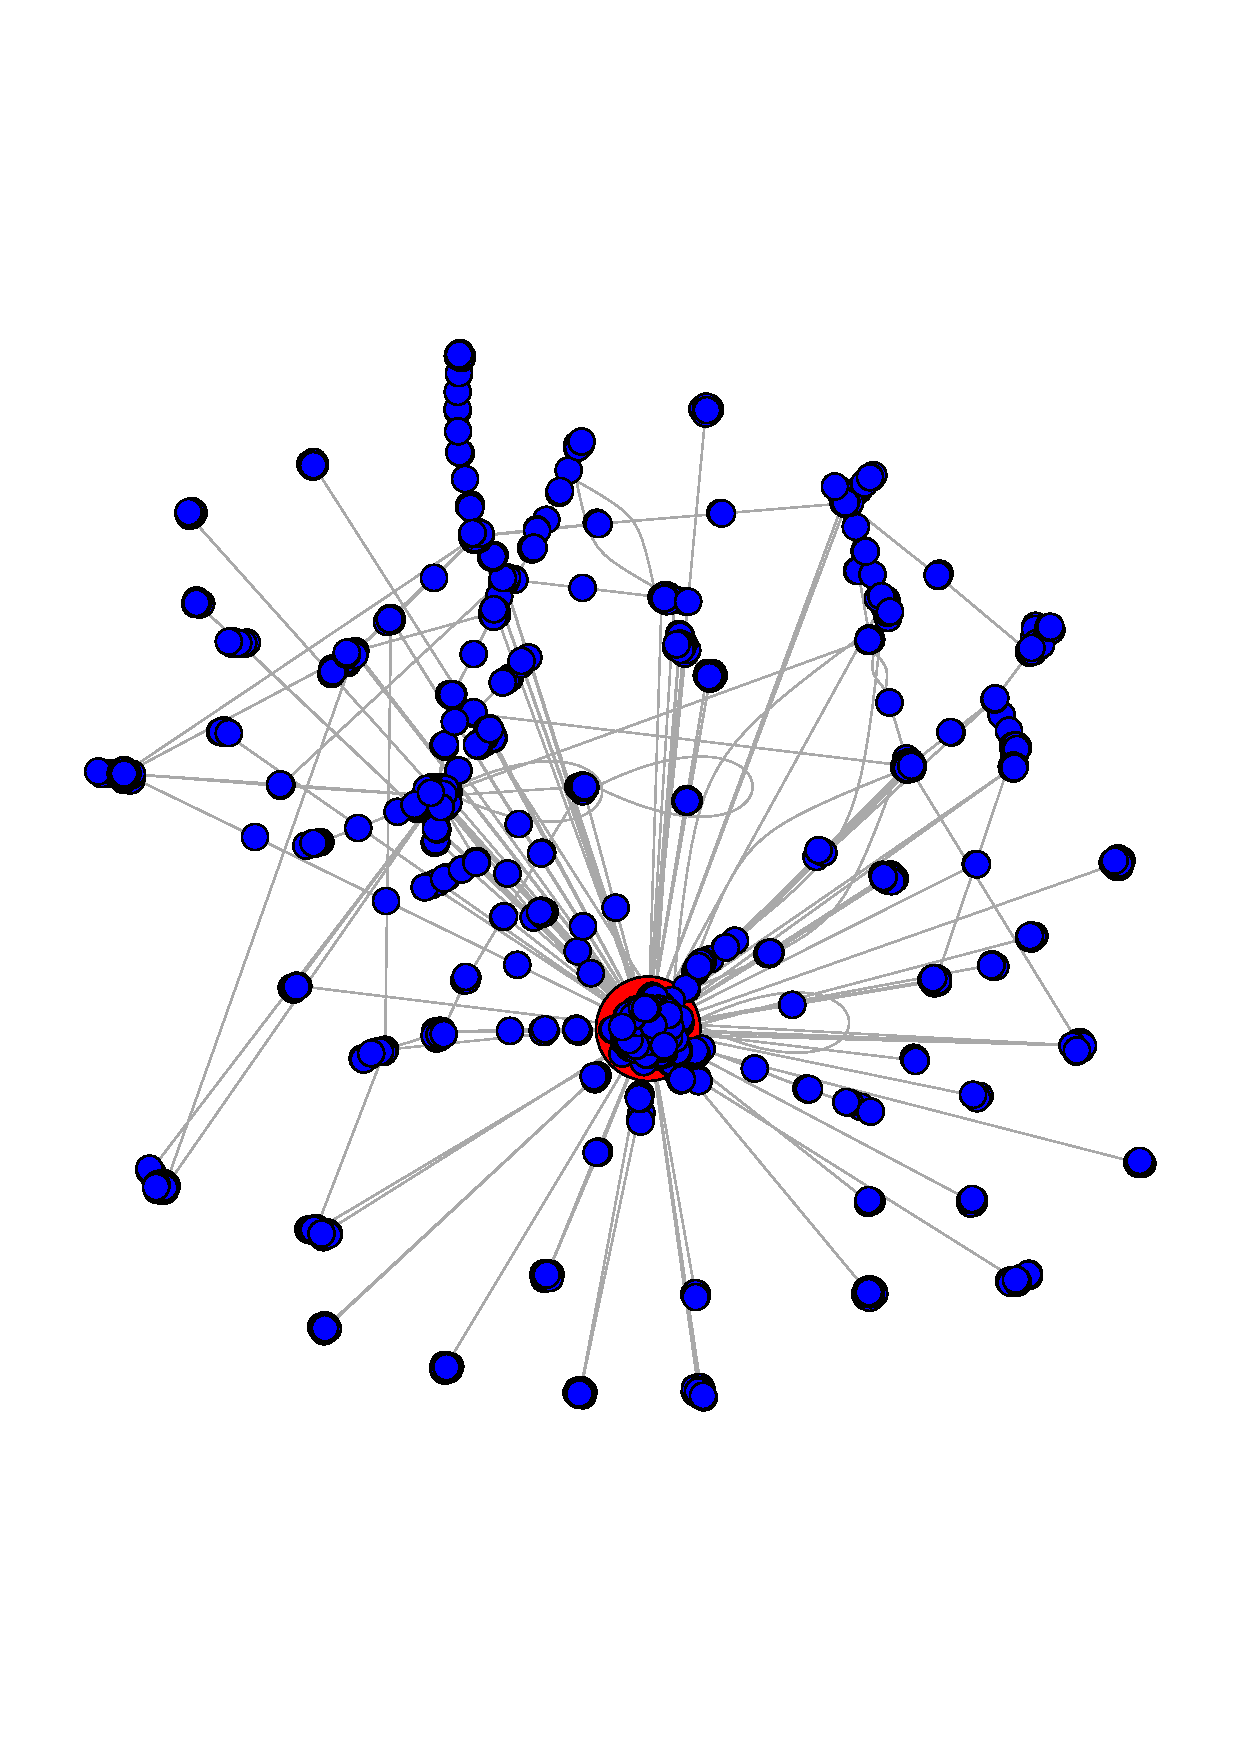
\includegraphics[width=0.95\linewidth]{/Users/mateuszzaremba/dev/R/Networks/Network/size colour node degree} \end{center}

The graph becomes even more readable when we use colouring to represent
the node's score of closeness and the node's sizing to represent its
measure of betweenness:

\begin{center}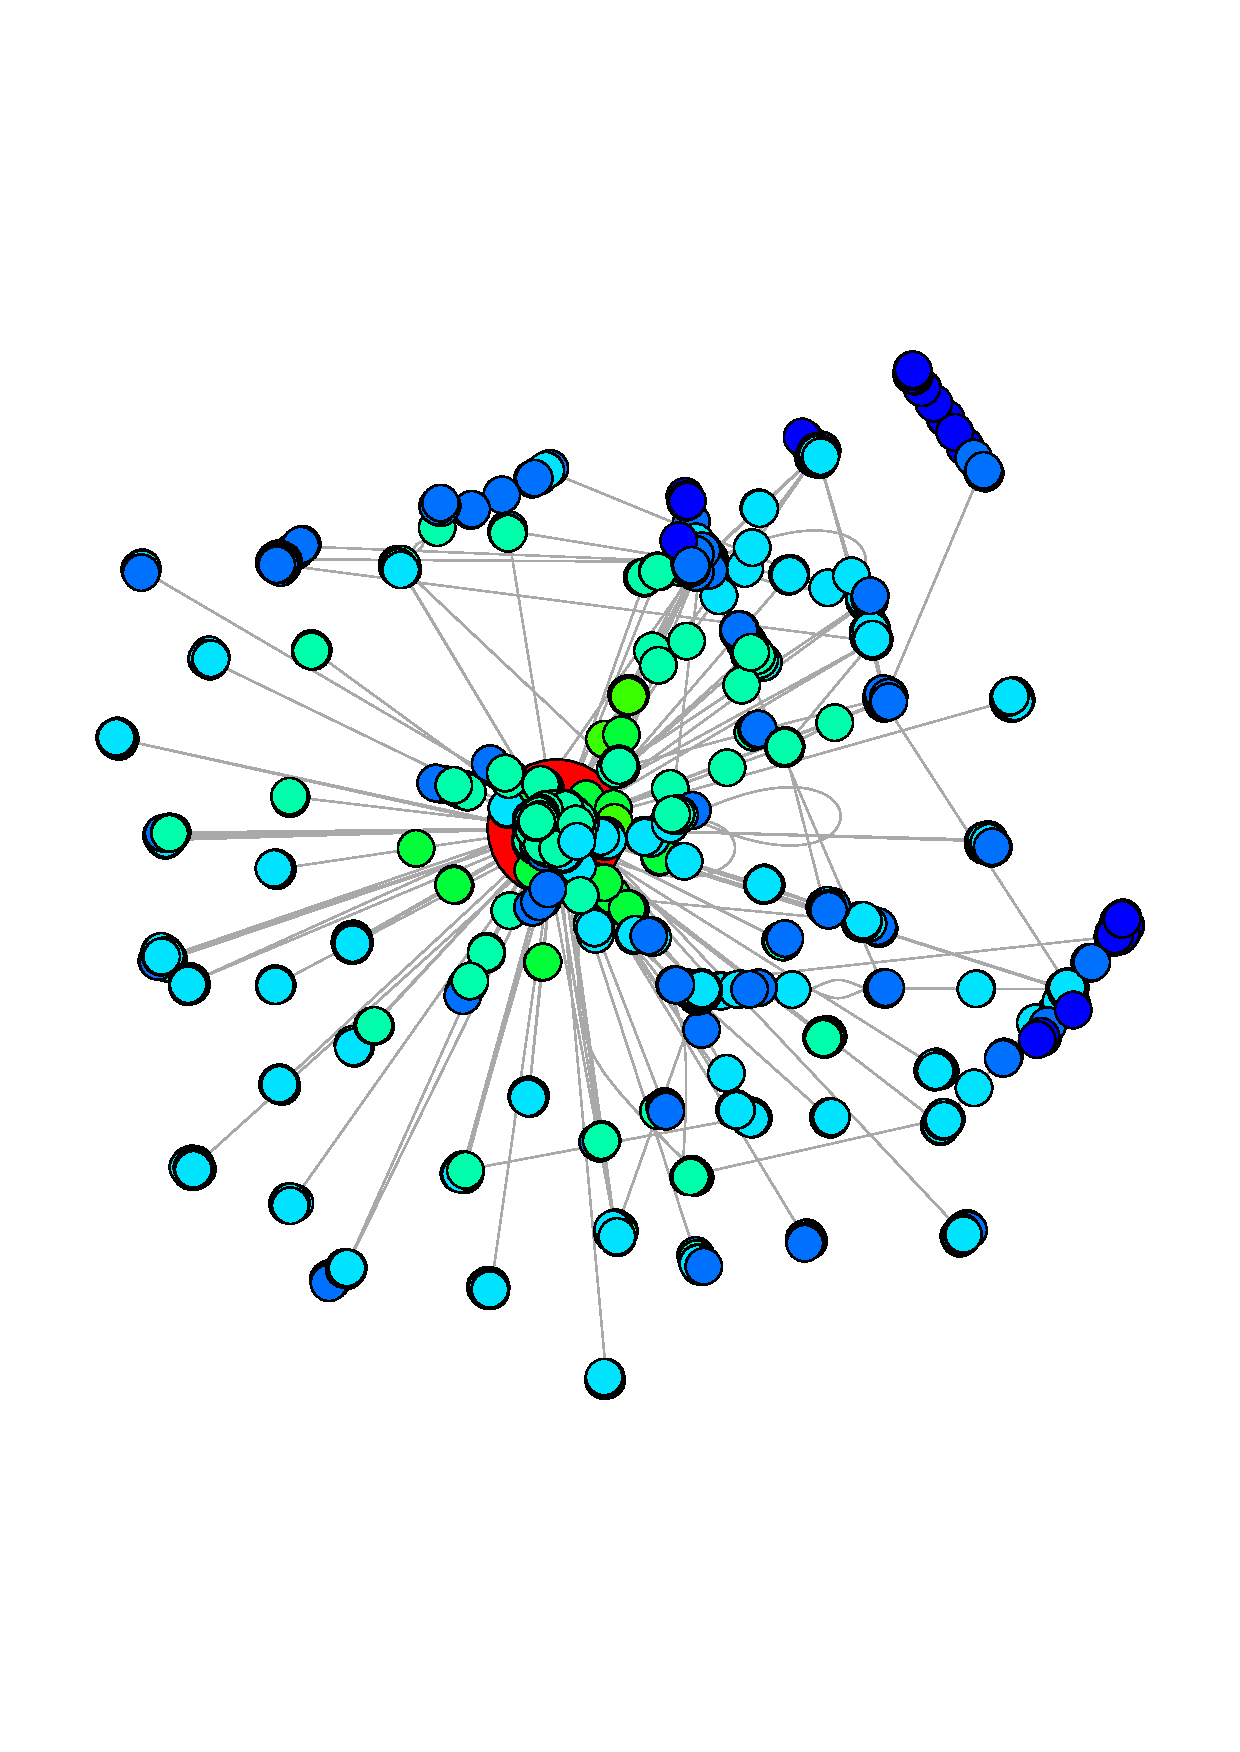
\includegraphics[width=0.95\linewidth]{/Users/mateuszzaremba/dev/R/Networks/Network/colour closeness - size betweenness with NO lgl} \end{center}

The same graph was plotted using \texttt{Large\ Graph\ Layout} function
which slightly improved the readability of the graph:

\begin{center}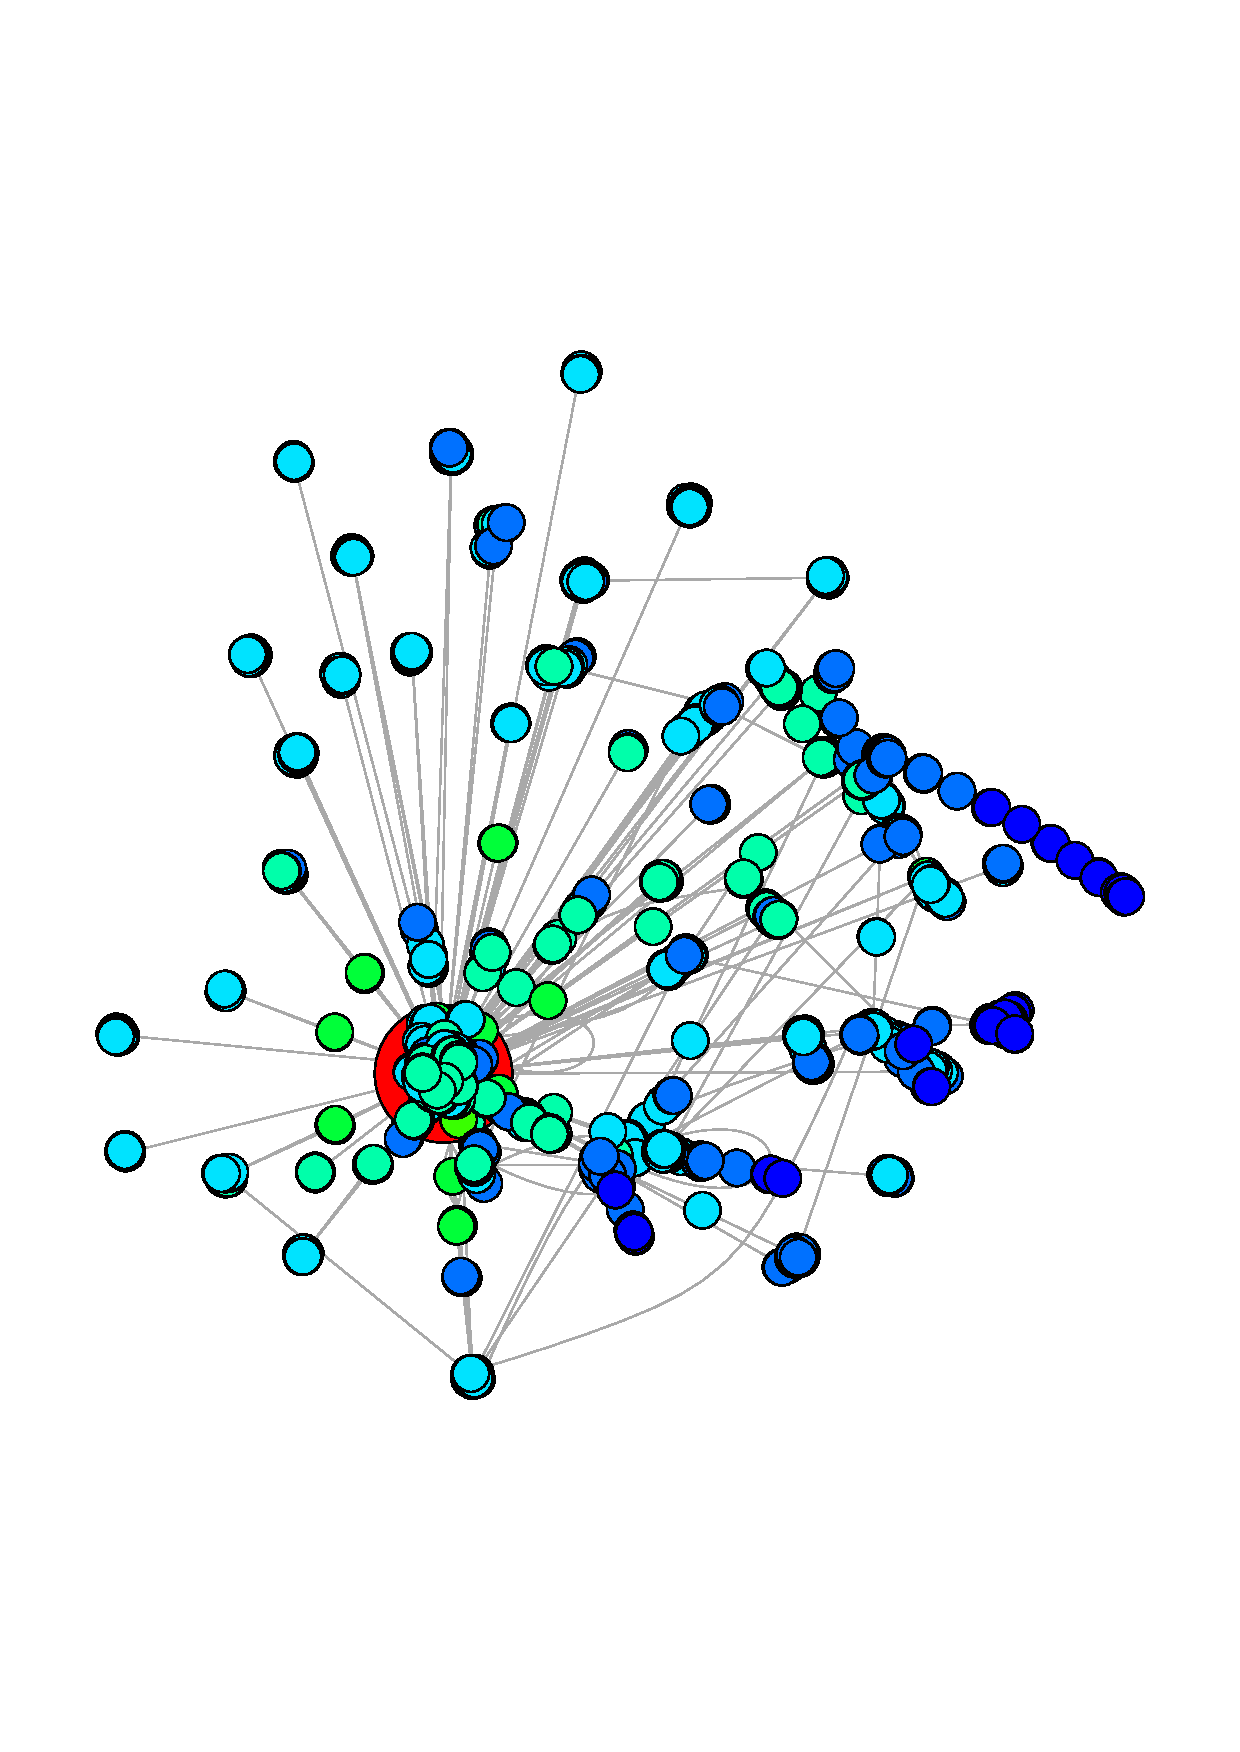
\includegraphics[width=0.95\linewidth]{/Users/mateuszzaremba/dev/R/Networks/Network/colour closeness - size betweenness with lgl} \end{center}

Interesting results were achieved using \texttt{Gephi} (Gephi.org,
2019), were it is clearly visible that there is one central node in the
network (Barack Obama):

\begin{center}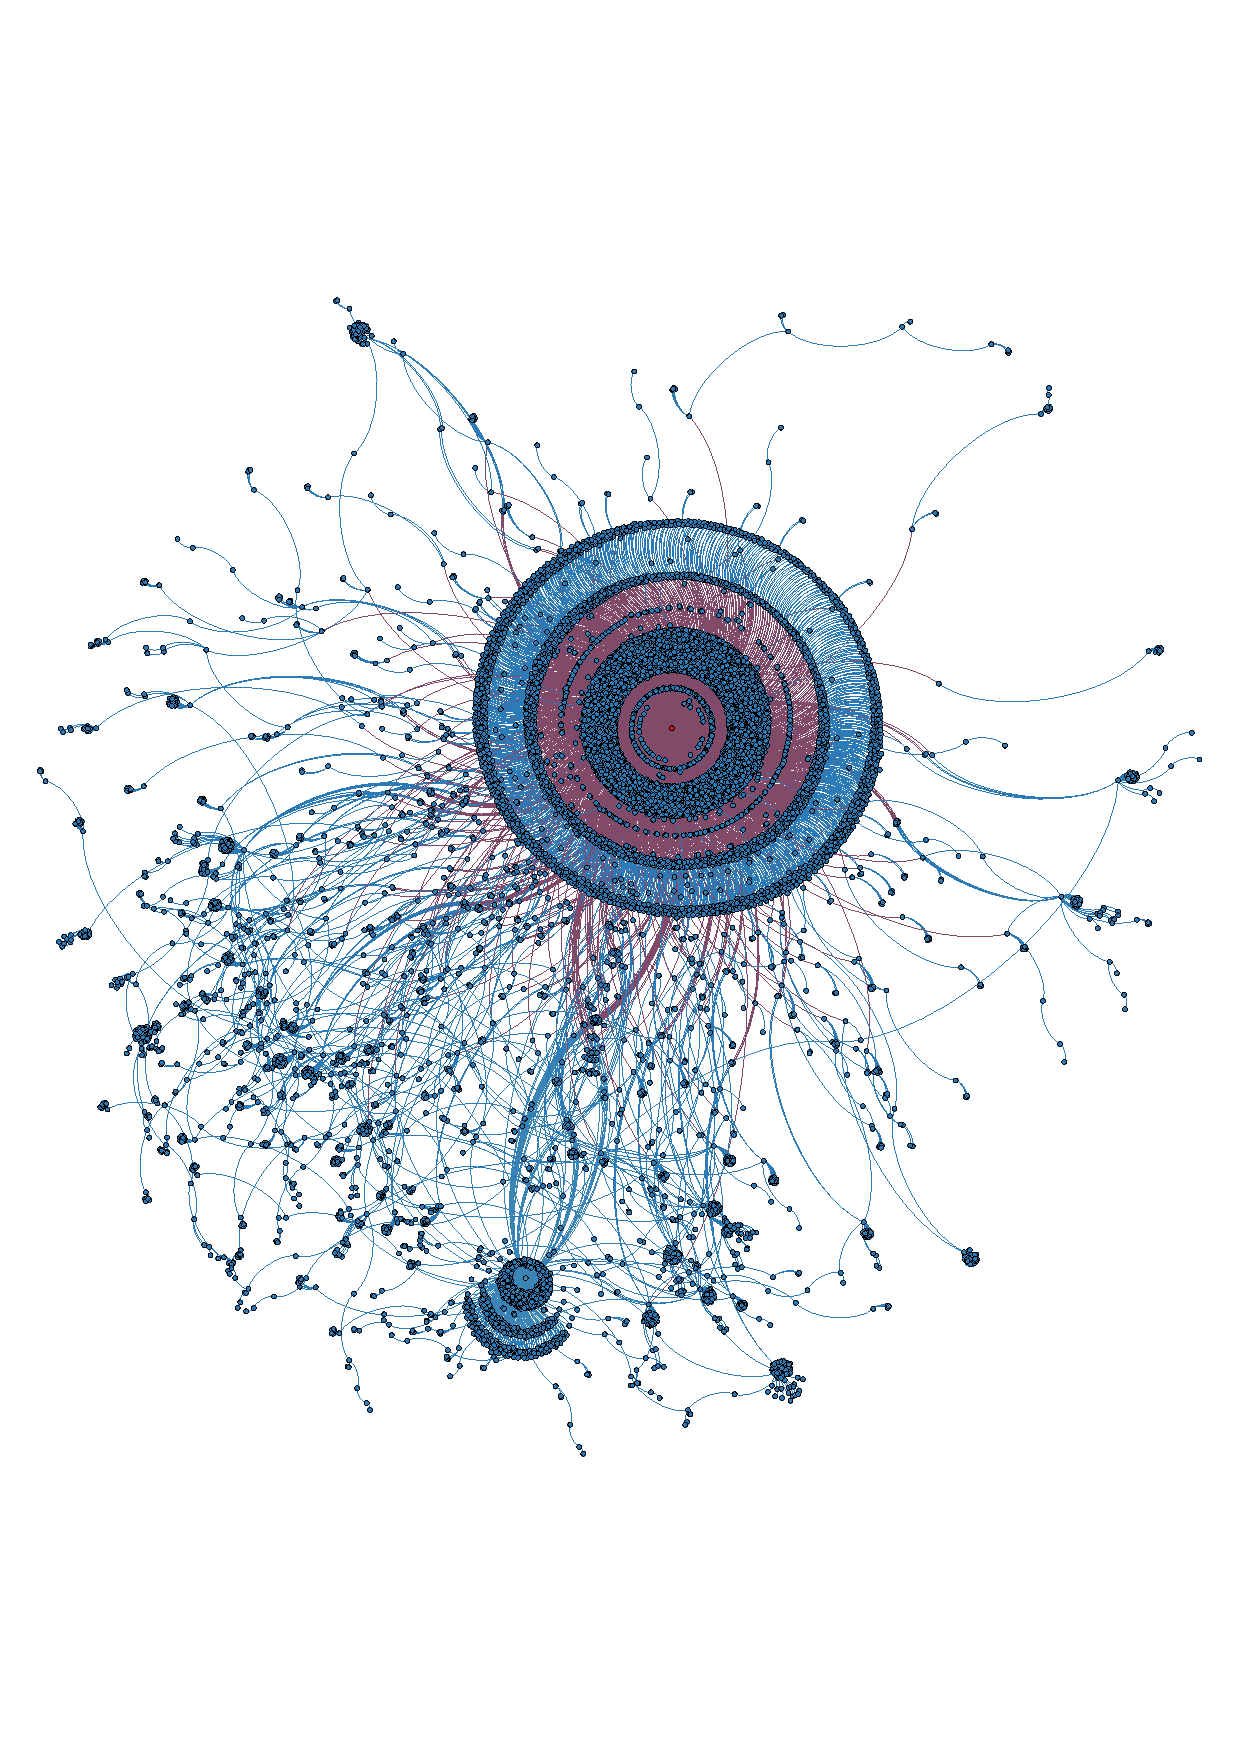
\includegraphics[width=0.95\linewidth]{/Users/mateuszzaremba/dev/R/Networks/pdf/gephi} \end{center}

And for the final proof, here is a zoom of the same graph generated with
Gephi and node labels on, where it is clearly visible that the most
central node, has an id of 2506:

\begin{center}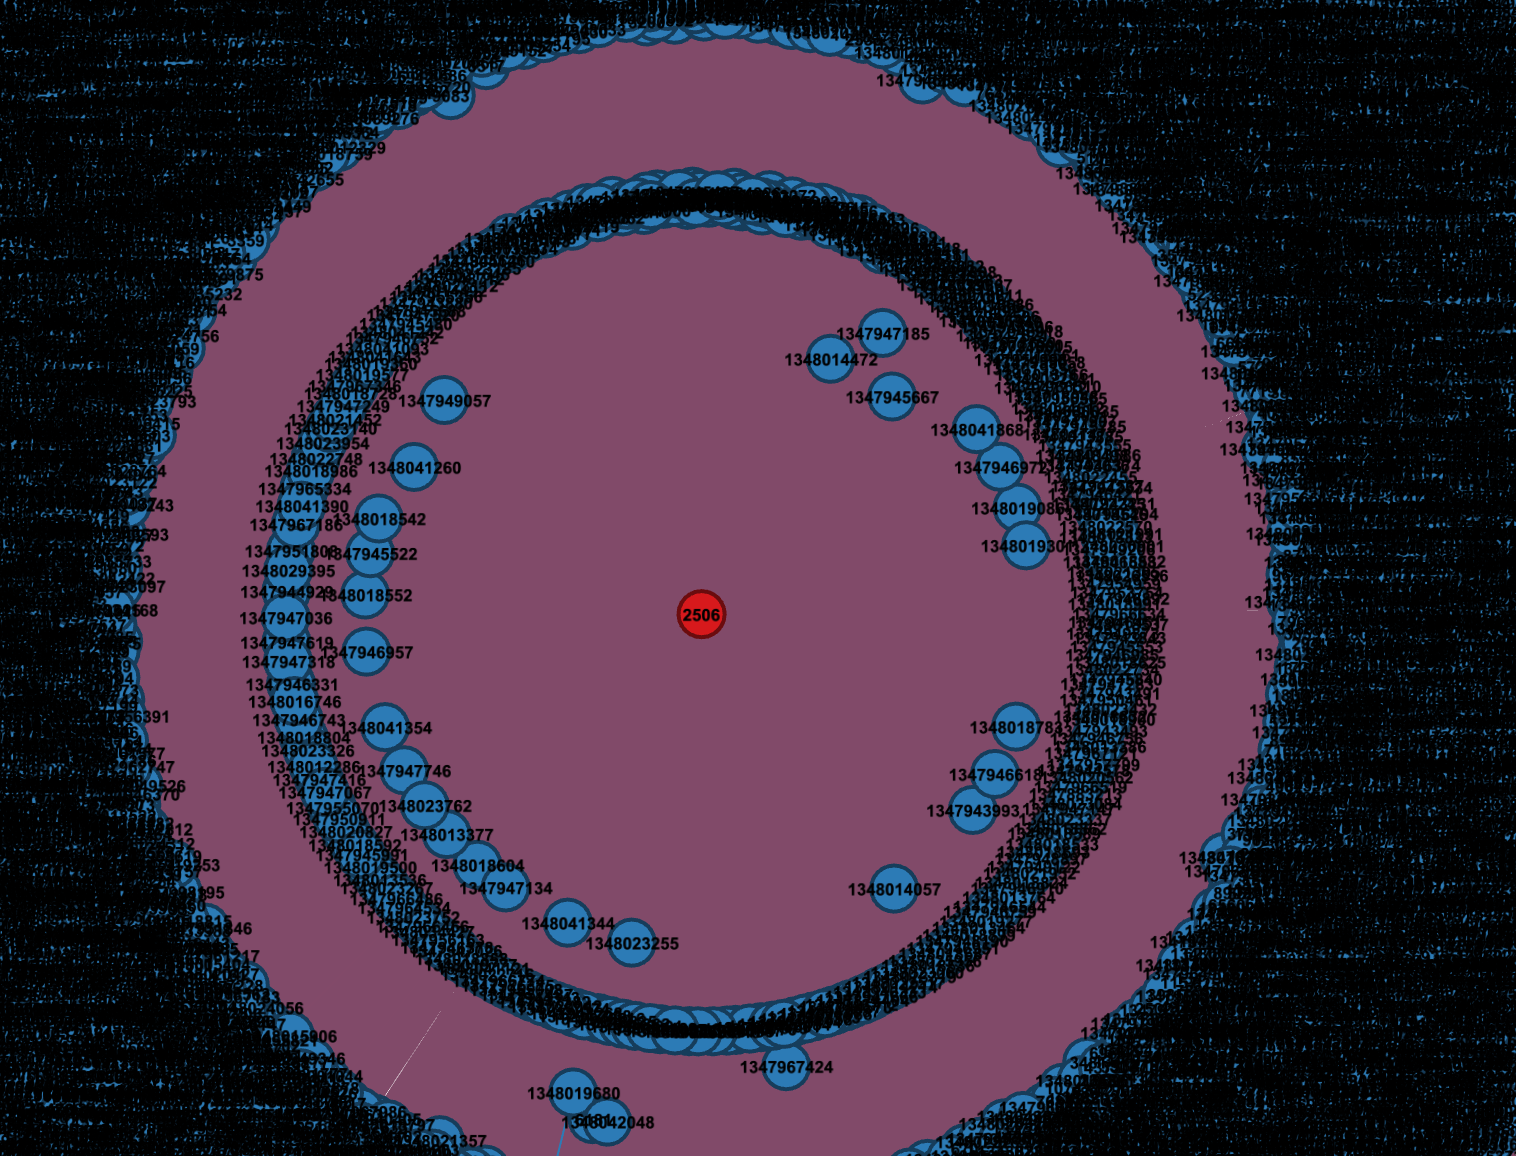
\includegraphics[width=1.00\linewidth]{/Users/mateuszzaremba/Desktop/Screenshot 2019-12-17 at 19.01.19} \end{center}

\hypertarget{conclusion}{%
\section{Conclusion}\label{conclusion}}

We managed to successfully identify the node which is very likely to be
Barack Obama's twitter account -- the nodes id was 2506; find the
shortest path between top two nodes with the highest degrees as well as
the node with the highest and the lowest degree; identify 138
communities within the network and their range; calculate and analyse
the network's closeness, betweenness and eigenvector centrality; conduct
a comprehensive visual analysis.

The size of the network proved it quite difficult to work with;
calculation of the node betweenness and closeness centrality took
approx. 40 minutes. Plotting of the network in R took only a few moments
but it was only due to the fact that the nodes' labels were not being
displayed, otherwise, it was taking approx. 5-10 minutes to plot.
Nonetheless, an attempt was made to speed up the process using
\texttt{with\_lgl(\ldots{})} (Rdrr.io, 2019) function for
\texttt{Large\ Graph\ Layout} (See Appendix B) but no improvement in
rendering speed was noticed apart from a slightly better visual
representation of the communities.

One of the things that could be done in the future, to improve
calculation and render times, when analysing as big or even bigger
networks, could be a usage of a GPU for network analysis.
(Mathworks.com, 2019); e.g.~Geforce GTS 250 has 450 cores working in
parallel versus 4 on the CPU (Kajan and Slačka, 2019).

Overall, the data was well described and of a good quality; the original
analysis provided a lot of good insight (Look table 1) and the size of
the data was appropriate for a comprehensive analysis.

\pagebreak

\hypertarget{references}{%
\section{References}\label{references}}

Gephi.org. (2019). Gephi - The Open Graph Viz Platform. {[}online{]}
Available at: \url{https://gephi.org/} {[}Accessed 16 Dec.~2019{]}.

Kajan, S. and Slačka, J. (2019). COMPUTING OF NEURAL NETWORK ON GRAPHICS
CARD. BSc. Slovak University of Technology in Bratislava.

Mathworks.com. (2019). Neural Networks with Parallel and GPU Computing-
MATLAB \& Simulink. {[}online{]} Available at:
\url{https://www.mathworks.com/help/deeplearning/ug/neural-networks-with-parallel-and-gpu-computing.html;jsessionid=fad53e284f66e53b4d2665c85a87}
{[}Accessed 16 Dec.~2019{]}.

Rdrr.io. (2019). layout\_with\_lgl: Large Graph Layout in igraph:
Network Analysis and Visualization. {[}online{]} Available at:
\url{https://rdrr.io/cran/igraph/man/layout_with_lgl.html} {[}Accessed
16 Dec.~2019{]}.

Rossi, R. and Ahmed, N. (2015). The Network Data Repository with
Interactive Graph Analytics and Visualization. {[}online{]} Network
Repository. Available at:
\url{http://networkrepository.com/rt-barackobama.php} {[}Accessed 16
Dec.~2019{]}.

Sci.unich.it. (2019). Betweenness Centrality. {[}online{]} Available at:
\url{https://www.sci.unich.it/~francesc/teaching/network/betweeness.html}
{[}Accessed 16 Dec.~2019{]}.

Sciencedirect.com. (2019). Closeness Centrality - an overview \textbar{}
ScienceDirect Topics. {[}online{]} Available at:
\url{https://www.sciencedirect.com/topics/computer-science/closeness-centrality}
{[}Accessed 16 Dec.~2019{]}.

Stack Overflow. (2019). Using networkx to calculate eigenvector
centrality. {[}online{]} Available at:
\url{https://stackoverflow.com/questions/43208737/using-networkx-to-calculate-eigenvector-centrality}
{[}Accessed 16 Dec.~2019{]}.

Sadler, J. (2019). Introduction to Network Analysis with R. {[}online{]}
Jesse Sadler. Available at:
\url{https://www.jessesadler.com/post/network-analysis-with-r/}
{[}Accessed 16 Dec.~2019{]}.

\pagebreak

\hypertarget{appendix-a}{%
\section{Appendix A}\label{appendix-a}}

Python code

\begin{Shaded}
\begin{Highlighting}[]
\ImportTok{import}\NormalTok{ networkx }\ImportTok{as}\NormalTok{ nx}
\ImportTok{import}\NormalTok{ csv}
\ImportTok{import}\NormalTok{ matplotlib.pyplot }\ImportTok{as}\NormalTok{ plt}
\ImportTok{from}\NormalTok{ operator }\ImportTok{import}\NormalTok{ itemgetter}
\ImportTok{from}\NormalTok{ matplotlib.pyplot }\ImportTok{import}\NormalTok{ figure}

\NormalTok{BO\_graph }\OperatorTok{=}\NormalTok{ nx.Graph()}
\ControlFlowTok{with} \BuiltInTok{open}\NormalTok{(}\StringTok{\textquotesingle{}barack\_obama.csv\textquotesingle{}}\NormalTok{,}\StringTok{\textquotesingle{}r\textquotesingle{}}\NormalTok{) }\ImportTok{as}\NormalTok{ BO:}
\NormalTok{  columns }\OperatorTok{=} \BuiltInTok{next}\NormalTok{(BO, }\VariableTok{None}\NormalTok{)}\CommentTok{\# skip the header row}
\NormalTok{  BO\_graph }\OperatorTok{=}\NormalTok{ nx.parse\_edgelist(BO, delimiter}\OperatorTok{=}\StringTok{\textquotesingle{},\textquotesingle{}}\NormalTok{, create\_using}\OperatorTok{=}\NormalTok{nx.Graph(),}
\NormalTok{    nodetype}\OperatorTok{=}\BuiltInTok{str}\NormalTok{, data}\OperatorTok{=}\NormalTok{((}\StringTok{\textquotesingle{}type\textquotesingle{}}\NormalTok{,}\BuiltInTok{str}\NormalTok{),(}\StringTok{\textquotesingle{}weight\textquotesingle{}}\NormalTok{, }\BuiltInTok{float}\NormalTok{),(}\StringTok{\textquotesingle{}book\textquotesingle{}}\NormalTok{,}\BuiltInTok{int}\NormalTok{)))}

\CommentTok{\# 1. Network size metrics}
\CommentTok{\# This will print the network\textquotesingle{}s:}
\CommentTok{\# {-} Number of edges}
\CommentTok{\# {-} Number of nodes}
\CommentTok{\# {-} Average degree}
\BuiltInTok{print}\NormalTok{(nx.info(BO\_graph))}

\CommentTok{\# 2. Network structure metrics}
\CommentTok{\# degree(\textquotesingle{}node id\textquotesingle{}, node degree)}
\NormalTok{highest\_degree }\OperatorTok{=} \BuiltInTok{max}\NormalTok{(BO\_graph.degree(), key}\OperatorTok{=}\KeywordTok{lambda}\NormalTok{ x : x[}\DecValTok{1}\NormalTok{])}
\NormalTok{sorted\_degree }\OperatorTok{=} \BuiltInTok{sorted}\NormalTok{(BO\_graph.degree(), key}\OperatorTok{=}\KeywordTok{lambda}\NormalTok{ x : x[}\DecValTok{1}\NormalTok{], reverse}\OperatorTok{=}\VariableTok{True}\NormalTok{)}
\BuiltInTok{print}\NormalTok{(}\StringTok{\textquotesingle{}Top 10 highest degrees:\textquotesingle{}}\NormalTok{, sorted\_degree[:}\DecValTok{10}\NormalTok{])}
\BuiltInTok{print}\NormalTok{(}\StringTok{\textquotesingle{}Highest degree:\textquotesingle{}}\NormalTok{, highest\_degree)}

\CommentTok{\# 3. Network Density}
\NormalTok{density }\OperatorTok{=}\NormalTok{ nx.density(BO\_graph)}
\BuiltInTok{print}\NormalTok{(}\StringTok{\textquotesingle{}Network density is:\textquotesingle{}}\NormalTok{, density)}

\CommentTok{\# 4. Shortest Path Between Two Nodes}
\CommentTok{\# 4.1 Shortest Path Between Top Two Highest Degree Nodes}
\CommentTok{\# Find ids of top 2 nodes with the highest degree}
\NormalTok{top\_two\_degree\_path }\OperatorTok{=}\NormalTok{ nx.shortest\_path(}
\NormalTok{  BO\_graph, source}\OperatorTok{=}\NormalTok{sorted\_degree[}\DecValTok{0}\NormalTok{][}\DecValTok{0}\NormalTok{], target}\OperatorTok{=}\NormalTok{sorted\_degree[}\DecValTok{1}\NormalTok{][}\DecValTok{0}\NormalTok{])}

\BuiltInTok{print}\NormalTok{(}\SpecialStringTok{f\textquotesingle{}Shortest path between node }\SpecialCharTok{\{}\NormalTok{sorted\_degree[}\DecValTok{0}\NormalTok{][}\DecValTok{0}\NormalTok{]}\SpecialCharTok{\}}\SpecialStringTok{\textbackslash{}}
\SpecialStringTok{  and node }\SpecialCharTok{\{}\NormalTok{sorted\_degree[}\DecValTok{1}\NormalTok{][}\DecValTok{0}\NormalTok{]}\SpecialCharTok{\}}\SpecialStringTok{:\textquotesingle{}}\NormalTok{, top\_two\_degree\_path)}
\BuiltInTok{print}\NormalTok{(}\StringTok{\textquotesingle{}Length of this path:\textquotesingle{}}\NormalTok{, }\BuiltInTok{len}\NormalTok{(top\_two\_degree\_path)}\OperatorTok{{-}}\DecValTok{1}\NormalTok{)}

\CommentTok{\# 4.2 Shortest Path Between Nodes With The Highest and The Loewst Degree}
\NormalTok{highest\_lowest\_degree\_path }\OperatorTok{=}\NormalTok{ nx.shortest\_path(}
\NormalTok{  BO\_graph, source}\OperatorTok{=}\NormalTok{sorted\_degree[}\DecValTok{0}\NormalTok{][}\DecValTok{0}\NormalTok{], target}\OperatorTok{=}\NormalTok{sorted\_degree[}\OperatorTok{{-}}\DecValTok{1}\NormalTok{][}\DecValTok{0}\NormalTok{])}

\BuiltInTok{print}\NormalTok{(}\SpecialStringTok{f\textquotesingle{}Shortest path between node with the highest degree of\textbackslash{}}
\SpecialStringTok{  }\SpecialCharTok{\{}\NormalTok{sorted\_degree[}\DecValTok{0}\NormalTok{][}\DecValTok{1}\NormalTok{]}\SpecialCharTok{\}}\SpecialStringTok{ and the node with the lowest degree of\textbackslash{} }
\SpecialStringTok{  }\SpecialCharTok{\{}\NormalTok{sorted\_degree[}\OperatorTok{{-}}\DecValTok{1}\NormalTok{][}\DecValTok{1}\NormalTok{]}\SpecialCharTok{\}}\SpecialStringTok{:\textquotesingle{}}\NormalTok{,}
\NormalTok{  highest\_lowest\_degree\_path)}
\BuiltInTok{print}\NormalTok{(}\StringTok{\textquotesingle{}Length of this path:\textquotesingle{}}\NormalTok{, }\BuiltInTok{len}\NormalTok{(highest\_lowest\_degree\_path)}\OperatorTok{{-}}\DecValTok{1}\NormalTok{)}

\CommentTok{\# 5. Improving the network visualisation}
\ImportTok{import}\NormalTok{ community}

\ImportTok{from}\NormalTok{ collections }\ImportTok{import}\NormalTok{ Counter}

\NormalTok{parts }\OperatorTok{=}\NormalTok{ community.best\_partition(BO\_graph)}
\NormalTok{values }\OperatorTok{=}\NormalTok{ [parts.get(node) }\ControlFlowTok{for}\NormalTok{ node }\KeywordTok{in}\NormalTok{ BO\_graph.nodes()]}

\BuiltInTok{print}\NormalTok{(Counter(values))}
\BuiltInTok{print}\NormalTok{(}\SpecialStringTok{f"Sizes of the communities range from\textbackslash{}}
\SpecialStringTok{  }\SpecialCharTok{\{}\BuiltInTok{min}\NormalTok{(Counter(values).items(), key}\OperatorTok{=}\KeywordTok{lambda}\NormalTok{ i : i[}\DecValTok{1}\NormalTok{])}\SpecialCharTok{\}}\SpecialStringTok{"}\NormalTok{)}
\BuiltInTok{print}\NormalTok{(}\SpecialStringTok{f"to }\SpecialCharTok{\{}\BuiltInTok{max}\NormalTok{(Counter(values).items(), key}\OperatorTok{=}\KeywordTok{lambda}\NormalTok{ i : i[}\DecValTok{1}\NormalTok{])}\SpecialCharTok{\}}\SpecialStringTok{"}\NormalTok{)}

\CommentTok{\# 6.    Network Structure Connectivity}
\ControlFlowTok{if}\NormalTok{ nx.is\_connected(BO\_graph):}
    \BuiltInTok{print}\NormalTok{(}\StringTok{"Barack Obama network is fully connected and has no sub{-}networks"}\NormalTok{)}
\ControlFlowTok{else}\NormalTok{:}
    \BuiltInTok{print}\NormalTok{(}\StringTok{"Barack Obama network is NOT fully connected"}\NormalTok{)}

\CommentTok{\# \# 7. Network Hubs/Brokers}
\CommentTok{\# 7.1 Node betweenness}
\NormalTok{betweenness\_dict }\OperatorTok{=}\NormalTok{ nx.betweenness\_centrality(BO\_graph)}

\CommentTok{\# Assign each to an attribute in your network}
\NormalTok{nx.set\_node\_attributes(BO\_graph, betweenness\_dict, }\StringTok{\textquotesingle{}betweenness\textquotesingle{}}\NormalTok{)}

\NormalTok{sorted\_betweenness }\OperatorTok{=} \BuiltInTok{sorted}\NormalTok{(betweenness\_dict.items(), }
\NormalTok{  key}\OperatorTok{=}\NormalTok{itemgetter(}\DecValTok{1}\NormalTok{), }
\NormalTok{  reverse}\OperatorTok{=}\VariableTok{True}\NormalTok{)}

\BuiltInTok{print}\NormalTok{(}\StringTok{"Top 20 nodes by betweenness centrality:"}\NormalTok{)}
\ControlFlowTok{for}\NormalTok{ i }\KeywordTok{in}\NormalTok{ sorted\_betweenness[:}\DecValTok{20}\NormalTok{]:}
    \BuiltInTok{print}\NormalTok{(i)}
\CommentTok{\# (\textquotesingle{}2506\textquotesingle{}, 0.9894963970281675)}
\CommentTok{\# (\textquotesingle{}9302\textquotesingle{}, 0.12282820504741454)}
\CommentTok{\# (\textquotesingle{}4143\textquotesingle{}, 0.03144816600031404)}
\CommentTok{\# ...}

\CommentTok{\# \# 7.2 Node closeness}
\NormalTok{closeness\_dict }\OperatorTok{=}\NormalTok{ nx.closeness\_centrality(BO\_graph)}

\CommentTok{\# Assign each to an attribute in your network}
\NormalTok{nx.set\_node\_attributes(BO\_graph, closeness\_dict, }\StringTok{\textquotesingle{}closeness\textquotesingle{}}\NormalTok{)}

\NormalTok{sorted\_closeness }\OperatorTok{=} \BuiltInTok{sorted}\NormalTok{(closeness\_dict.items(), }
\NormalTok{  key}\OperatorTok{=}\NormalTok{itemgetter(}\DecValTok{1}\NormalTok{), }
\NormalTok{  reverse}\OperatorTok{=}\VariableTok{True}\NormalTok{)}

\BuiltInTok{print}\NormalTok{(}\StringTok{"Top 20 nodes by closeness centrality:"}\NormalTok{)}
\ControlFlowTok{for}\NormalTok{ i }\KeywordTok{in}\NormalTok{ sorted\_closeness[:}\DecValTok{20}\NormalTok{]:}
    \BuiltInTok{print}\NormalTok{(i)}
\CommentTok{\# (\textquotesingle{}2506\textquotesingle{}, 0.6994988014818043)}
\CommentTok{\# (\textquotesingle{}6675\textquotesingle{}, 0.4373297002724796)}
\CommentTok{\# (\textquotesingle{}8744\textquotesingle{}, 0.4362993838347227)}
\CommentTok{\# ...}

\CommentTok{\# \# 7.3 Node eigenvector centrailty}
\CommentTok{\# using: nx.eigenvector\_centrality()}
\CommentTok{\# error: PowerIterationFailedConvergence: }
\CommentTok{\# (PowerIterationFailedConvergence(...), }
\CommentTok{\# \textquotesingle{}power iteration failed to converge within 100 iterations\textquotesingle{})}
\CommentTok{\# use: nx.eigenvector\_centrality\_numpy()}
\NormalTok{eigenvector\_dict }\OperatorTok{=}\NormalTok{ nx.eigenvector\_centrality\_numpy(BO\_graph)}

\NormalTok{nx.set\_node\_attributes(BO\_graph, eigenvector\_dict, }\StringTok{\textquotesingle{}eigenvector\textquotesingle{}}\NormalTok{)}

\NormalTok{sorted\_eigenvector }\OperatorTok{=} \BuiltInTok{sorted}\NormalTok{(eigenvector\_dict.items(), }
\NormalTok{  key}\OperatorTok{=}\NormalTok{itemgetter(}\DecValTok{1}\NormalTok{), }
\NormalTok{  reverse}\OperatorTok{=}\VariableTok{True}\NormalTok{)}

\BuiltInTok{print}\NormalTok{(}\StringTok{"Top 20 nodes by eigenvector centrality:"}\NormalTok{)}
\ControlFlowTok{for}\NormalTok{ b }\KeywordTok{in}\NormalTok{ sorted\_eigenvector[:}\DecValTok{20}\NormalTok{]:}
    \BuiltInTok{print}\NormalTok{(b)}
\CommentTok{\# Top 20 nodes by eigenvector centrality:}
\CommentTok{\# (\textquotesingle{}2506\textquotesingle{}, 0.7070870193199195)}
\CommentTok{\# (\textquotesingle{}8983\textquotesingle{}, 0.00849854648835321)}
\CommentTok{\# (\textquotesingle{}8744\textquotesingle{}, 0.008303338474194982)}
\CommentTok{\# ...}
\end{Highlighting}
\end{Shaded}

\pagebreak

\hypertarget{appendix-b}{%
\section{Appendix B}\label{appendix-b}}

R code

\begin{Shaded}
\begin{Highlighting}[]
\KeywordTok{library}\NormalTok{(igraph)}
\KeywordTok{library}\NormalTok{(tidyverse)}
\KeywordTok{library}\NormalTok{(ggraph)}
\KeywordTok{library}\NormalTok{(tidygraph)}

\CommentTok{\# download}
\NormalTok{pth <{-}}\StringTok{ "http://nrvis.com/download/data/rt/rt\_barackobama.zip"}
\KeywordTok{download.file}\NormalTok{(pth, }\DataTypeTok{destfile =} \StringTok{"rt\_barackobama.zip"}\NormalTok{)}

\CommentTok{\# see file names}
\KeywordTok{unzip}\NormalTok{(}\StringTok{"rt\_barackobama.zip"}\NormalTok{, }\DataTypeTok{list =} \OtherTok{TRUE}\NormalTok{)}

\CommentTok{\# unzip}
\NormalTok{unz <{-}}\StringTok{ }\KeywordTok{unzip}\NormalTok{(}\StringTok{"rt\_barackobama.zip"}\NormalTok{, }\StringTok{"rt\_barackobama.edges"}\NormalTok{)}

\NormalTok{dat <{-}}\StringTok{ }\KeywordTok{read.table}\NormalTok{(unz, }\DataTypeTok{sep=}\StringTok{","}\NormalTok{)}

\CommentTok{\# Drop 3rd column (V3) of the dataframe because it\textquotesingle{}s only a timestamp}
\NormalTok{dat <{-}}\StringTok{ }\KeywordTok{select}\NormalTok{(dat,}\OperatorTok{{-}}\KeywordTok{c}\NormalTok{(}\DecValTok{3}\NormalTok{))}

\CommentTok{\# Rename}
\NormalTok{dat <{-}}\StringTok{ }\NormalTok{dat }\OperatorTok{\%>\%}
\StringTok{  }\KeywordTok{rename}\NormalTok{(}
    \DataTypeTok{from =}\NormalTok{ V1,}
    \DataTypeTok{to =}\NormalTok{ V2}
\NormalTok{  )}

\CommentTok{\# Save as csv to use in python}
\KeywordTok{write.csv}\NormalTok{(dat,}\StringTok{"barack\_obama.csv"}\NormalTok{, }\DataTypeTok{row.names =} \OtherTok{FALSE}\NormalTok{)}

\CommentTok{\# Create graph}
\NormalTok{g <{-}}\StringTok{ }\KeywordTok{graph\_from\_data\_frame}\NormalTok{(dat, }\DataTypeTok{directed=}\OtherTok{FALSE}\NormalTok{)}
\KeywordTok{summary}\NormalTok{(g)}

\CommentTok{\# Ensure that that the plots take most of the available page space}
\KeywordTok{par}\NormalTok{(}\DataTypeTok{oma=}\KeywordTok{c}\NormalTok{(}\DecValTok{0}\NormalTok{,}\DecValTok{0}\NormalTok{,}\DecValTok{0}\NormalTok{,}\DecValTok{0}\NormalTok{),}\DataTypeTok{mar=}\KeywordTok{c}\NormalTok{(}\DecValTok{0}\NormalTok{,}\DecValTok{0}\NormalTok{,}\DecValTok{0}\NormalTok{,}\DecValTok{0}\NormalTok{))}

\CommentTok{\# Colour the nodes based on their degree}
\NormalTok{colors.new=}\KeywordTok{rev}\NormalTok{(}\KeywordTok{rainbow}\NormalTok{(}\KeywordTok{max}\NormalTok{(}\KeywordTok{degree}\NormalTok{(g))}\OperatorTok{+}\DecValTok{1}\NormalTok{,}\DataTypeTok{end=}\DecValTok{2}\OperatorTok{/}\DecValTok{3}\NormalTok{))}
\KeywordTok{V}\NormalTok{(g)}\OperatorTok{$}\NormalTok{color=colors.new[}\KeywordTok{degree}\NormalTok{(g)}\OperatorTok{+}\DecValTok{1}\NormalTok{]}
\KeywordTok{plot.igraph}\NormalTok{(g,}\DataTypeTok{vertex.label=}\OtherTok{NA}\NormalTok{)}

\CommentTok{\# Set vertex size according to degree of each vertex (min. size = 5)}
\KeywordTok{V}\NormalTok{(g)}\OperatorTok{$}\NormalTok{size=}\DecValTok{5}\OperatorTok{+}\NormalTok{(}\DecValTok{15}\NormalTok{)}\OperatorTok{/}\KeywordTok{diff}\NormalTok{(}\KeywordTok{range}\NormalTok{(}\KeywordTok{degree}\NormalTok{(g)))}\OperatorTok{*}\KeywordTok{degree}\NormalTok{(g)}
\CommentTok{\# Plot the graph without node labels}
\KeywordTok{plot.igraph}\NormalTok{(g,}\DataTypeTok{vertex.label=}\OtherTok{NA}\NormalTok{)}

\CommentTok{\# Set nodes\textquotesingle{} colour palette for clossness centrality}
\CommentTok{\# creates a color palette for us to use}
\NormalTok{colors.new=}\KeywordTok{rev}\NormalTok{(}\KeywordTok{rainbow}\NormalTok{(}\DecValTok{10}\NormalTok{,}\DataTypeTok{end=}\DecValTok{4}\OperatorTok{/}\DecValTok{6}\NormalTok{)) }
\CommentTok{\# calculates closeness metric for all nodes}
\NormalTok{net.close=}\KeywordTok{as.numeric}\NormalTok{(}\KeywordTok{closeness}\NormalTok{(g)) }
\CommentTok{\# normalises the closeness value}
\NormalTok{net.close=}\KeywordTok{floor}\NormalTok{((net.close}\OperatorTok{{-}}\KeywordTok{min}\NormalTok{(net.close))}\OperatorTok{/}
\StringTok{  }\KeywordTok{diff}\NormalTok{(}\KeywordTok{range}\NormalTok{(net.close))}\OperatorTok{*}\NormalTok{(}\KeywordTok{length}\NormalTok{(colors.new)}\OperatorTok{{-}}\DecValTok{1}\NormalTok{)}\OperatorTok{+}\DecValTok{1}\NormalTok{) }
\CommentTok{\# sets the color of each node according to the closenss score}
\KeywordTok{V}\NormalTok{(g)}\OperatorTok{$}\NormalTok{color=colors.new[net.close] }
\CommentTok{\# Plot the graph without node labels}
\KeywordTok{plot.igraph}\NormalTok{(g,}\DataTypeTok{vertex.label=}\OtherTok{NA}\NormalTok{)}

\CommentTok{\# Ser node size for betweenness centrality}
\CommentTok{\# calculates betweenness of each node}
\NormalTok{net.between=}\KeywordTok{as.numeric}\NormalTok{(}\KeywordTok{betweenness}\NormalTok{(g))}
\CommentTok{\# "normalises" the score}
\NormalTok{net.between=}\KeywordTok{floor}\NormalTok{((net.between}\OperatorTok{{-}}\KeywordTok{min}\NormalTok{(net.between))}\OperatorTok{/}
\StringTok{  }\KeywordTok{diff}\NormalTok{(}\KeywordTok{range}\NormalTok{(net.between))}\OperatorTok{*}\NormalTok{(}\KeywordTok{length}\NormalTok{(colors.new)}\OperatorTok{{-}}\DecValTok{1}\NormalTok{)}\OperatorTok{+}\DecValTok{1}\NormalTok{) }
\CommentTok{\# sets the node size accoring the betweenness score}
\KeywordTok{V}\NormalTok{(g)}\OperatorTok{$}\NormalTok{size=}\DecValTok{5}\OperatorTok{+}\NormalTok{(}\DecValTok{20}\NormalTok{)}\OperatorTok{/}\KeywordTok{diff}\NormalTok{(}\KeywordTok{range}\NormalTok{(net.between))}\OperatorTok{*}\NormalTok{net.between }
\CommentTok{\# Plot the graph without node labels}
\KeywordTok{plot.igraph}\NormalTok{(g,}\DataTypeTok{vertex.label=}\OtherTok{NA}\NormalTok{)}

\CommentTok{\# Layout for big graphs}
\NormalTok{area <{-}}\StringTok{ }\KeywordTok{vcount}\NormalTok{(g)}\OperatorTok{\^{}}\DecValTok{2}
\KeywordTok{layout\_with\_lgl}\NormalTok{(g, }\DataTypeTok{maxiter =} \DecValTok{150}\NormalTok{, }\DataTypeTok{maxdelta =} \KeywordTok{vcount}\NormalTok{(g),}
  \DataTypeTok{area =} \KeywordTok{vcount}\NormalTok{(g)}\OperatorTok{\^{}}\DecValTok{2}\NormalTok{, }\DataTypeTok{coolexp =} \FloatTok{1.5}\NormalTok{, }\DataTypeTok{repulserad =}\NormalTok{ area }\OperatorTok{*}
\StringTok{  }\KeywordTok{vcount}\NormalTok{(g), }\DataTypeTok{cellsize =} \KeywordTok{sqrt}\NormalTok{(}\KeywordTok{sqrt}\NormalTok{(area)), }\DataTypeTok{root =} \OtherTok{NULL}\NormalTok{)}

\CommentTok{\# Plot g with lgl and without node labels}
\KeywordTok{with\_lgl}\NormalTok{(}\KeywordTok{plot.igraph}\NormalTok{(g, }\DataTypeTok{vertex.label=}\OtherTok{NA}\NormalTok{))}
\end{Highlighting}
\end{Shaded}


\end{document}
